\section{力矩~转动惯量~定轴转动定律}

\subsection{力矩}

\subsubsection{区分定点转动力矩和定轴转动力矩}

$$\mathbf{M}=\mathbf{r}\times\mathbf{F}$$

定点转动的力矩可以使物体在任意运动方向上改变状态。

而对于定轴转动，分解到平行于转轴的力不能改变转动状态，只有垂直于转轴的力才能改变刚体的转动状态，因此，定轴转动中可以改变转动状态的力矩分量与转轴平行。

\textbf{在定轴转动中，总力矩的量值等于多个力矩的代数和。}

\begin{figure}[h]
	\centering
	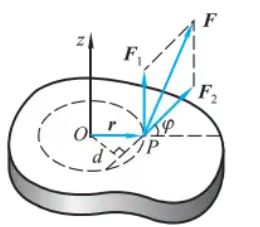
\includegraphics[width=0.3\linewidth]{images/力矩}
	\caption[定轴转动的力矩]{}
	\label{fig:}
\end{figure}
$\mathbf{F_1}$为平行于转轴的力，$\mathbf{F_2}$为垂直于转轴的力，d成为力臂。
$$ |\mathbf{M_z}|=|\mathbf{F_2}\mathbf{r}\sin\varphi|=|\mathbf{F_2}d|$$

\subsection{角速度}

1.角速度为\textbf{矢量}，$\mathbf{v}=\mathbf{\omega}\mathbf{r} $

2.角速度的方向用右手螺旋定则判断，且对于定轴转动，角速度方向始终与转轴平行。

\subsection{转动惯量和定轴转动定律}

下给出简要推导：

取刚体中任一质量元$\Delta m$,其受外力为$\mathbf{F_{ei}}$,受内力为$\mathbf{F_{i}}$

由牛顿第二定律$$\mathbf{F_{ei}}+\mathbf{F_{i}} ={\Delta m}\mathbf{a_i}$$

在自然坐标系中$${F_ei}\sin\varphi_i+F_{i}\sin\theta_i= \Delta m\mathbf{r_i}\mathbf{\alpha}$$

同乘$\mathbf{r_i}$，并对质量元累加$$\sum_{i=1}^{n}{F_{ei}}\sin\varphi_i+\sum_{i=1}^{n}F_{i}\sin\theta_i=\sum_{i=1}^{n}\Delta m_i{r_i}^2\alpha$$

对于刚体而言，内力作用产生的相对位移为0，因此内力矩之和为零。

因此$$\mathbf{M_z}=J\mathbf{\alpha}=J\dfrac{\mathrm{d\omega}}{\mathrm{d}t}$$
\begin{figure}[h]
	\centering
	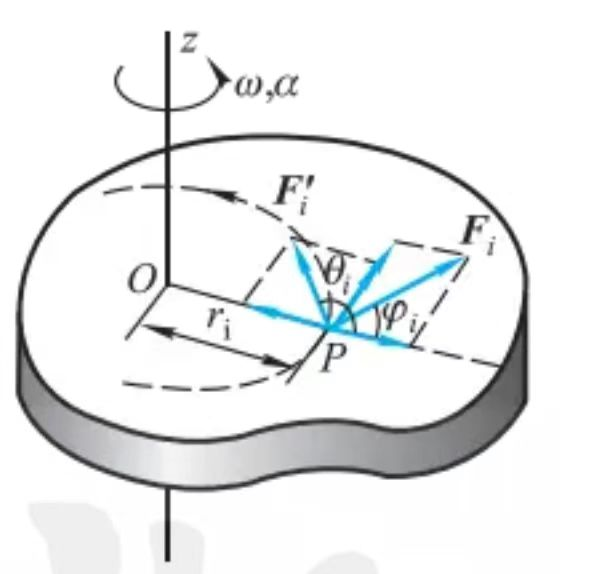
\includegraphics[width=0.3\linewidth]{images/定轴转动定律}
	\caption{定轴转动定律}
	\label{fig:}
\end{figure}

\subsubsection{转动惯量}

1.$J=\sum_{i=1}^{n}\Delta m_i{r_i}^2 $，单位为$kg\cdot m^2$

2.当刚体为质量连续体时，$J=\int r^2\mathrm{d}m $(其中r为质元$\mathrm{d}m $到轴的距离)

3.转动惯量取决于刚体的形状大小、质量分布和转轴的位置。

\subsubsection{转动与平动的联系}

对比牛顿第二定律和定轴转动定律
$\left\{
\begin{aligned}
	\mathbf{F}=m\mathbf{a}\\
	\mathbf{M}=\mathbf{J}\alpha
\end{aligned}
\right.$

其中，m成为惯性质量，是平动惯性的量度，而$\mathbf{J}$也可视作定轴转动刚体的一种特性，是刚体转动惯量的量度；且牛顿第二定律两边同乘$\mathbf{r}$,即为定轴转动定律，因此，可将定轴转动定律视作转动下的牛顿第二定律。

\subsubsection{平行轴定理}

\textbf{刚体对任一转轴的转动惯量$\mathbf{J}$等于通过质心轴的转动惯量$\mathbf{J_c}$加上$\mathbf{mh^2}$,其中$\mathbf{h}$ 为两平行轴之间的距离。}

$$\mathbf{J}=\int(x+h)^2\mathrm{d}m=\int x^2\mathrm{d}m+\int h^2\mathrm{d}m+2h\int x\mathrm{d}m=\mathbf{J_c}+mh^2 $$

(当刚体是绕定轴转动的匀质对称刚体时，$\int x\mathrm{d}m=0 $)

\subsubsection{常见模型的转动惯量}

下给出薄圆盘的转动惯量证明，刚体的转动惯量一般都可由一般模型和平行轴定理推导而得。

圆盘的质量为m,半径为R,设圆盘面密度为$\sigma$，则$\sigma=\dfrac{m}{\pi R^2}$,取宽度为$\mathrm{d}r $的圆环，则有该圆环质量$\mathrm{d}m=(2\pi r)\mathrm{d}r$,则
$$\mathbf{J}=\int r^2\mathrm{d}m=\int_{0}^{R}2\pi\sigma r^3\mathrm{d}r=\dfrac{\pi\sigma R^4}{2}=\frac{1}{2}mR^2$$

\begin{figure}[h]
	\centering
	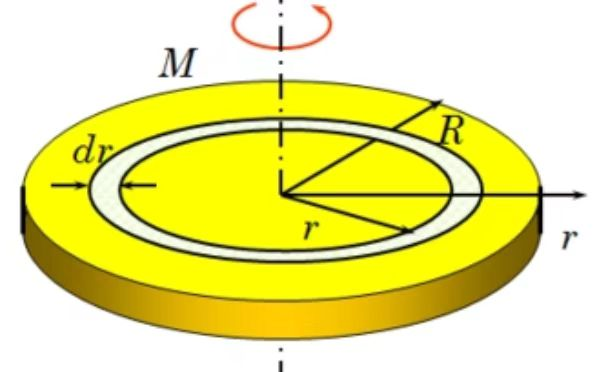
\includegraphics[width=0.2\linewidth]{images/薄圆盘转动惯量}
	\caption[薄圆盘转动惯量]{}
	\label{fig:}
\end{figure}
下为常见刚体转动惯量（书P118-119)
\begin{figure}[h]
	\centering
	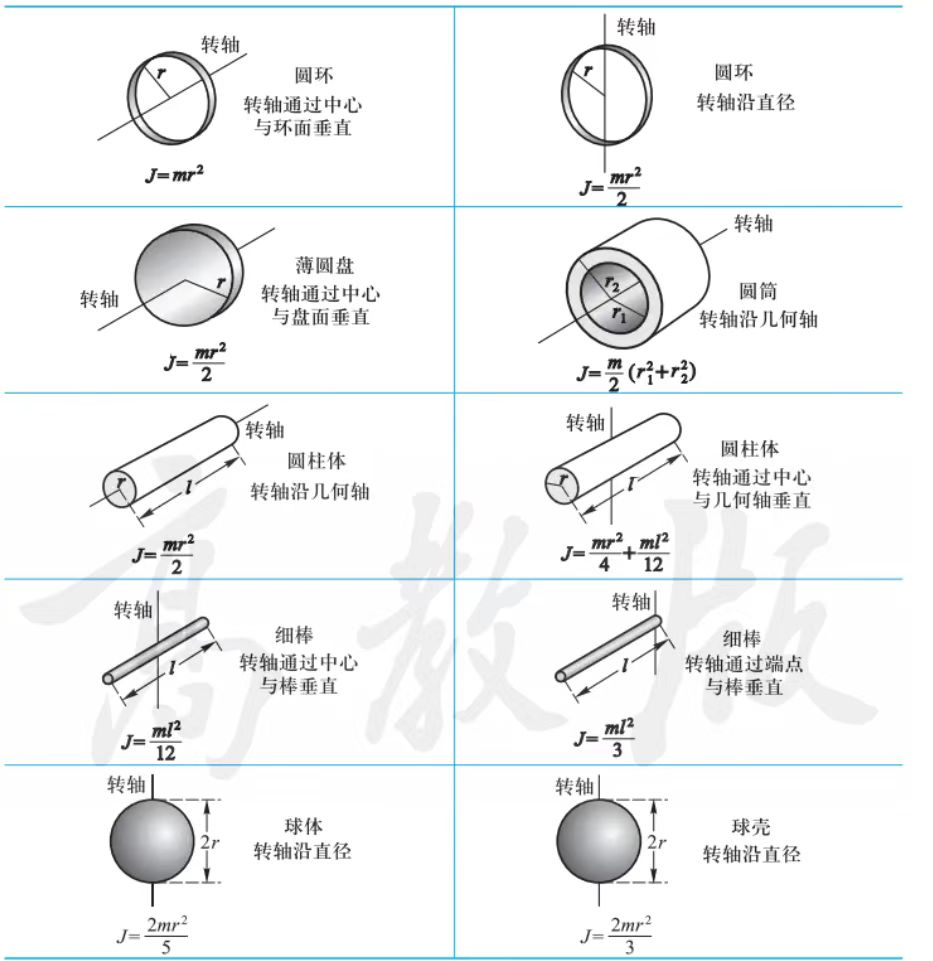
\includegraphics[width=0.9\linewidth]{images/转动惯量模型}
	\caption[转动惯量模型]{}
	\label{fig:}
\end{figure}
